%\documentclass{slides}
\documentclass{beamer}
\usepackage[utf8]{inputenc}
%\usepackage{portland}
\usepackage{graphicx}
%\usepackage{pdflscape}

%========Hierboven niets veranderen!========%

\usepackage[export]{adjustbox}% for the second solution
\usepackage{amsmath}
\usepackage{amsfonts}
\usepackage{amssymb}
\usepackage{bbding}
\usepackage{mathtools}
\usepackage{scalerel}
\usepackage[normalem]{ulem}
\usepackage{wisjab}

\setlength\fboxsep{4mm}
\setlength\fboxrule{0.8mm}

\definecolor{mygreen}{rgb}{0, 0.5, 0}
\def\gemph#1{{\color{mygreen}#1}}
\def\ck{\cellcolor{green!05}}

\def\lbt{} %Titel die linksboven verschijnt
\parindent=0pt
%\makesavenoteenv{tabular}
\renewcommand{\thefootnote}{\arabic{footnote}}

\def\d{\mathsf d}
\def\e{\mathsf e}
\def\i{\mathsf i}

\def\+{\kern0.0833em}
\def\:{\kern-0.07em}
\def\>{\kern0.08em}
\def\<{\kern-0.08em}

\renewcommand{\thefootnote}{\arabic{footnote}}

\newenvironment{dia}[2]
{
	\begin{frame}
	\vspace{1mm}
	{\small #1}
	\hfill
    {\small\bf\textcolor{blue}{#2}}
	\vspace{3mm}
	\hrule
	\bigskip
}
{
	\vfill
	\end{frame}
}

\frenchspacing

\begin{document}

\setlength{\abovedisplayskip}{3mm}
\setlength{\belowdisplayskip}{3mm}
\setlength{\abovedisplayshortskip}{3mm}
\setlength{\belowdisplayshortskip}{3mm}

\begin{dia}{\lbt}{}
\vspace*{0.5cm}
\begin{center}
\begin{large}
QA assessment Scholt Energy \\[1.25cm]
\end{large}
\begin{LARGE}
\textcolor{mygreen}{A game of Werewolves} \\[1.25cm]
\end{LARGE}
Dyon van Vreumingen
\end{center}
\end{dia}

\begin{dia}{\lbt}{Inhoud}
$ $\\
\begin{itemize}
    \setlength{\itemsep}{3mm}
    \item Formulering van weerwolven als stochastisch proces \pause
    \item Exacte oplossing voor het makkelijke geval (44 spelers) \pause
    \begin{itemize}
        \item Dynamisch programmeren \pause
    \end{itemize}
    \item Oplossingsrichtingen voor het moeilijke geval (veel spelers) \pause
    \begin{itemize}
        \item Continue meestervergelijking \pause
        \item Weerwolven als Itô-proces
    \end{itemize}
\end{itemize}
\vspace{1.6cm}
\end{dia}

\begin{dia}{\lbt}{}
\vspace{2.5cm}
\begin{center}
\begin{LARGE}
\textcolor{mygreen}{Weerwolven als stochastisch proces}
\end{LARGE}
\end{center}
\vspace*{1.5cm}
\end{dia}

\begin{dia}{\lbt}{Weerwolven}
Een groep spelers speelt samen weerwolven \pause \bigskip

Sommigen van de spelers zijn weerwolf, de rest dorpeling \smallskip

De dorpelingen weten niet wie de wolven zijn \pause \bigskip

Het spel wordt gespeeld over een aantal ronden. In elke ronde \pause
\begin{enumerate}[(1)]
    \item kiezen de wolven een dorpeling om op te eten \pause
    \item kiest de gehele groep een speler om te verwijderen \pause
\end{enumerate}
\bigskip

De wolven winnen als er geen dorpelingen meer over zijn \smallskip

De dorpelingen winnen als er geen wolven meer over zijn
\vspace{5mm}
\end{dia}

\begin{dia}{\lbt}{Weerwolven}
Een groep spelers speelt samen weerwolven \bigskip

Sommigen van de spelers zijn weerwolf, de rest dorpeling \smallskip

De dorpelingen weten niet wie de wolven zijn \bigskip

Het spel wordt gespeeld over een aantal ronden. In elke ronde
\begin{enumerate}[(1)]
    \item kiezen de wolven een dorpeling om op te eten
    \item kiest de gehele groep {\color{mygreen} uniform willekeurig} een speler om te verwijderen
\end{enumerate}
\bigskip

De wolven winnen als er geen dorpelingen meer over zijn \smallskip

De dorpelingen winnen als er geen wolven meer over zijn
\end{dia}

\begin{dia}{\lbt}{De vraag}
\vspace{2cm}
\begin{center}
    {\color{mygreen} Vraag}: \bigskip
    
    bij hoeveel wolven hebben de wolven en de dorpelingen (ongeveer) evenveel kans om te winnen?
\end{center}

\vspace{1.5cm}
\end{dia}

\begin{dia}{\lbt}{Wiskundige formulering}
We modelleren het spel als een \gemph{stochastisch proces} \pause \bigskip

Variabelen:
\begin{itemize}
    \item $t$: het aantal gespeelde rondes ($t = 0, 1, 2, 3, ...$) \pause
    \item $D_t$: het aantal dorpelingen dat na de $t$-de ronde over is \pause
    \item $W_t$: het aantal wolven dat na de $t$-de ronde over is \pause
    \item $D_0$: het aantal dorpelingen aan het begin van het spel \pause
    \item $W_0$: het aantal wolven aan het begin van het spel \pause
\end{itemize} \smallskip

Aannames:
\begin{itemize}
    \item we beginnen met een even aantal spelers ($D_0 + W_0$ is even) \pause
    \item we beginnen met meer dorpelingen dan wolven ($W_0 < D_0$)
\end{itemize}
\end{dia}

\begin{dia}{\lbt}{Wiskundige formulering}
We modelleren het spel als een \gemph{stochastisch proces} \bigskip

In elke ronde twee mogelijkheden: \pause
\begin{itemize}
    \item een dorpeling opgegeten en een dorpeling verwijderd: $D_t = D_{t-1} - 2$, $W_t = W_{t-1}$ \pause
    \item een dorpeling opgegeten en een wolf verwijderd: $D_t = D_{t-1} - 1$, $W_t = W_{t-1} - 1$
\end{itemize} \pause \bigskip

Dorpelingen winnen na de $t$-de ronde als $W_t = 0$ \pause \bigskip

Wolven winnen na de $t$-de ronde als $W_t = D_t$ \smallskip

(dorpelingen kunnen dan onmogelijk meer winnen!)
\end{dia}

\begin{dia}{\lbt}{Wiskundige formulering}
We modelleren het spel als een \gemph{stochastisch proces} \bigskip \bigskip

Kansverdeling:
\begin{align*}
    P(D_t = D_{t-1} - 2, W_t = W_{t-1}) &= \frac{D_{t-1} - 1}{D_{t-1} - 1 + W_{t-1}} \\[4mm]
    P(D_t = D_{t-1} - 1, W_t = W_{t-1} - 1) &= \frac{W_{t-1}}{D_{t-1} - 1 + W_{t-1}}
\end{align*}

\vspace{1cm}
\end{dia}

\begin{dia}{\lbt}{Nieuwe variabelen}
Twee stochastische variabelen ($D_t$ en $W_t$) bijhouden is onhandig \pause \bigskip

Daarom wissel van variabelen: \pause
\begin{itemize}
    \item $T_t = D_t + W_t$ (totaal aantal spelers na $t$ rondes)
    \item $\delta_t = D_t - W_t$ (verschil dorpelingen en wolven na $t$ rondes)
\end{itemize} \pause \bigskip

$T_t$ is bekend: elke ronde worden altijd 2 spelers verwijderd, dus $T_t = T_0 - 2t$ \pause \bigskip

Nu hebben we maar één stochastische variabele over, namelijk $\delta_t$
\end{dia}

\begin{dia}{\lbt}{Nieuwe variabelen}
Kansverdeling in termen van $\delta_t$:
\begin{align*}
    P(\delta_t = \delta_{t-1} - 2) &= p(\delta_{t - 1}, t - 1) \\[4mm]
    P(\delta_t = \delta_{t-1}) &= 1 - p(\delta_{t - 1}, t - 1)
\end{align*}
waarbij
\begin{align*}
    p(\delta, t) = \frac{\frac12\delta + \frac12T_0 - t - 1}{T_0 - 2t - 1}
\end{align*} \pause \smallskip

Dorpelingen winnen na $t$ rondes als $\delta_t = T_0 - 2t$ \pause \bigskip

Wolven winnen na $t$ rondes als $\delta_t = 0$
\vspace{-6mm}
\end{dia}

\begin{dia}{\lbt}{}
\vspace{2.5cm}
\begin{center}
\begin{LARGE}
\textcolor{mygreen}{Het makkelijke geval ($T_0$ = 44)}
\end{LARGE}
\end{center}
\vspace*{1.5cm}
\end{dia}

\begin{dia}{\lbt}{Kansen berekenen}
Eerste stap: wat is de kans dat de wolven na $t$ rondes winnen bij $T_0$ spelers en $W_0$ wolven? \pause \bigskip

We bepalen dit door de kansen $P(\delta_t = \delta)$ uit te rekenen \pause \bigskip

Als we dit weten, kunnen we de winkansen berekenen: \pause
\begin{align*}
    P(\text{wolven winnen}) &= \sum_t P(\delta_t = 0) \\[1mm]
    P(\text{dorpelingen winnen}) &= 1 - P(\text{wolven winnen})
\end{align*}

\pause Hiertoe gebruiken we de \gemph{meestervergelijking}:
\begin{align*}
    P(\delta_t = \delta) &= P(\delta_{t-1} = \delta + 2) \cdot p(\delta_{t-1}, t - 1) \\ 
    &+ P(\delta_{t-1} = \delta) \cdot [1 - p(\delta_{t-1}, t - 1)]
\end{align*}
\vspace{-2cm}
\end{dia}

\begin{dia}{\lbt}{Dynamisch programmeren}
Voorbeeld ($D_0 = 6, W_0 = 2 \Rightarrow T_0 = 8, \delta_0 = 4$)
\begin{center}
    
\includegraphics[width=0.75\textwidth]{fig/DP.png}
\end{center}
\vspace{-1.2cm}
\end{dia}

\begin{dia}{\lbt}{Binair zoeken}
We weten nu de winkansen $P_{\text{win}}(T_0, W_0)$. \smallskip

Maar hoe bepalen we het eerlijke aantal wolven? \pause \bigskip\bigskip

Bijvoorbeeld: alle $W_0$ afgaan en bepalen welke $P_{\text{win}}(T_0, W_0)$ het dichtst bij $\frac12$ zit \pause \bigskip\bigskip

Maar het kan slimmer met \gemph{binair zoeken}

\vspace{1.5cm}
\end{dia}

\begin{dia}{\lbt}{Binair zoeken}
\begin{center}
    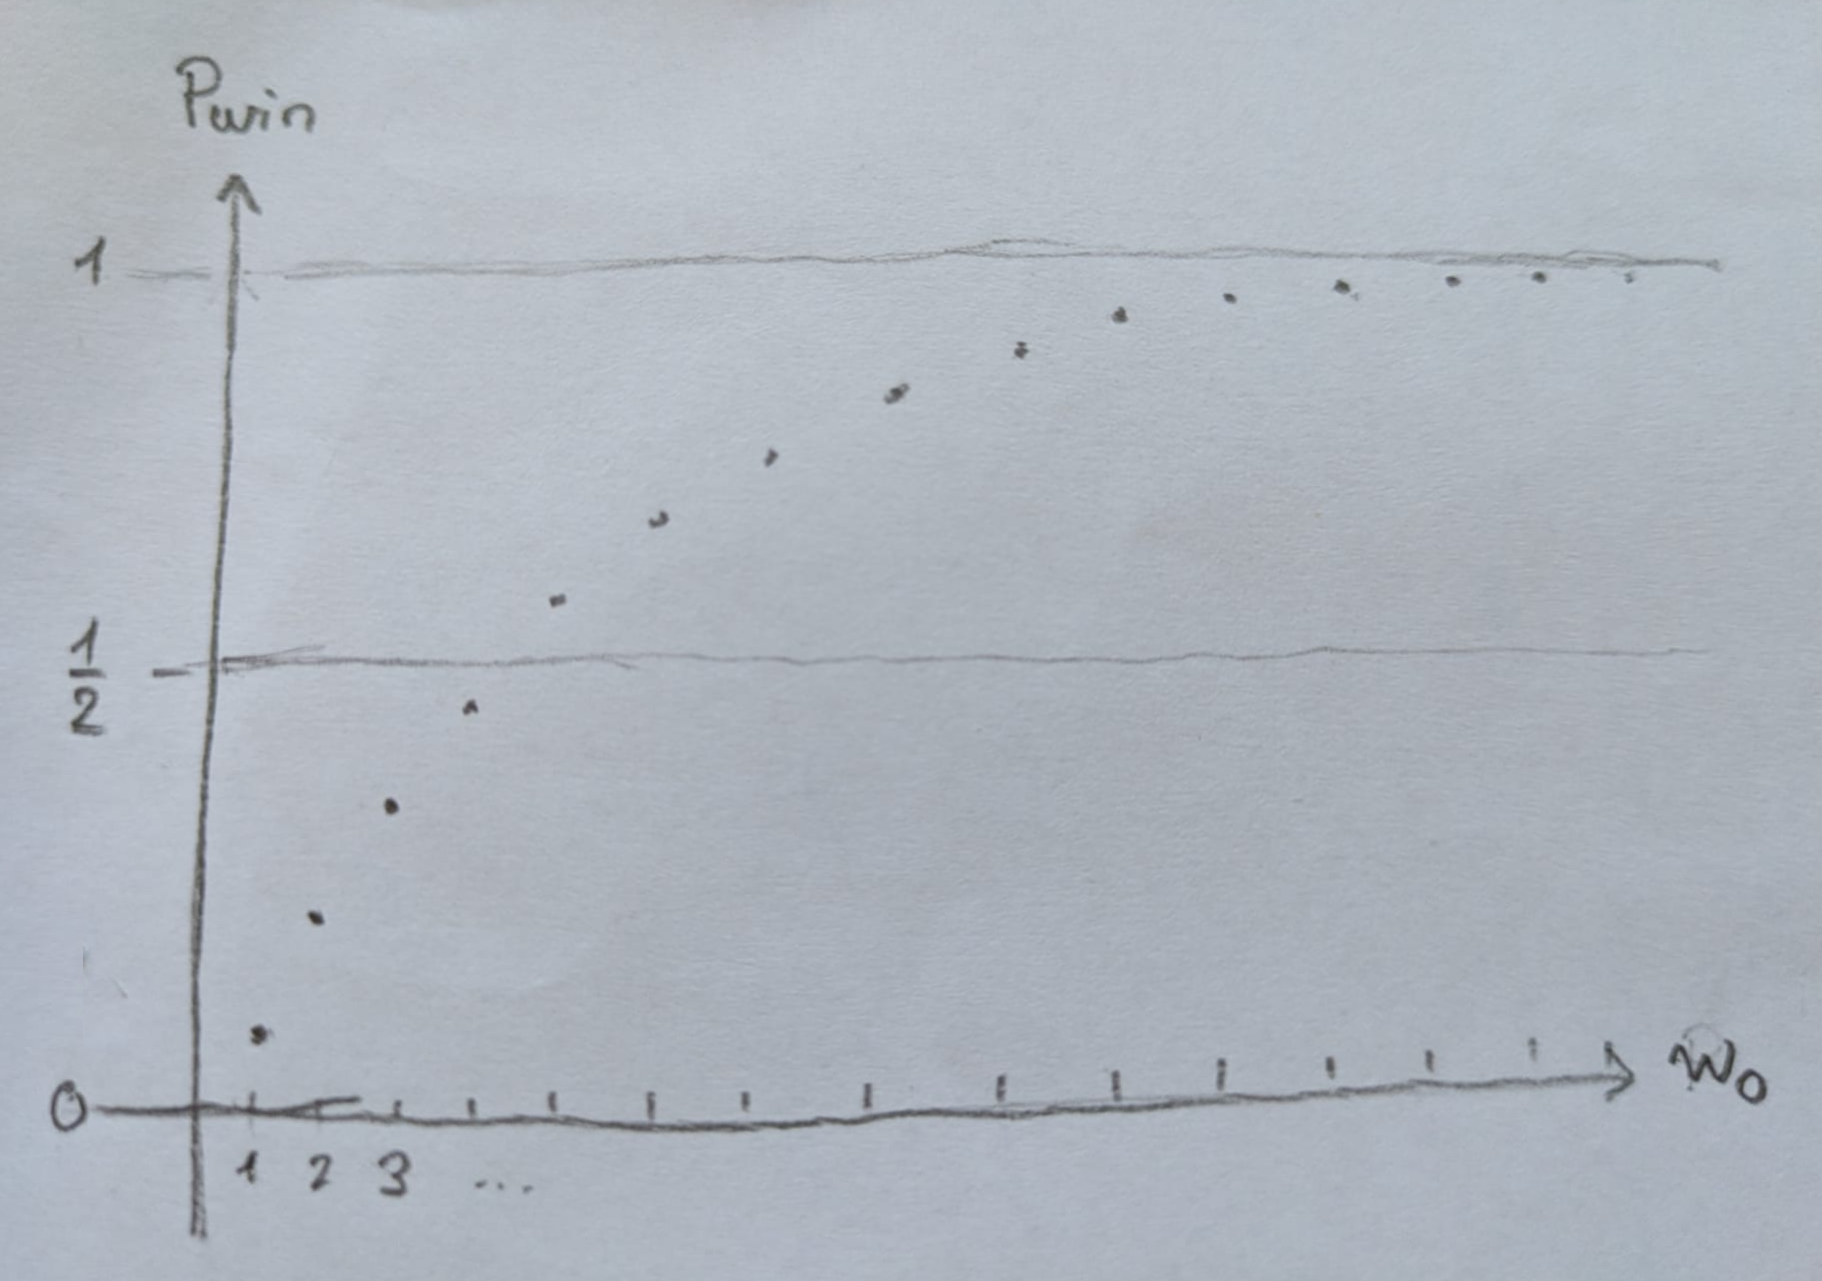
\includegraphics[width=0.9\textwidth]{fig/Binair.png}
\end{center}
\vspace{-1.5cm}
\end{dia}

\begin{dia}{\lbt}{Resultaat}
\vspace{0.2cm}
\begin{center}
    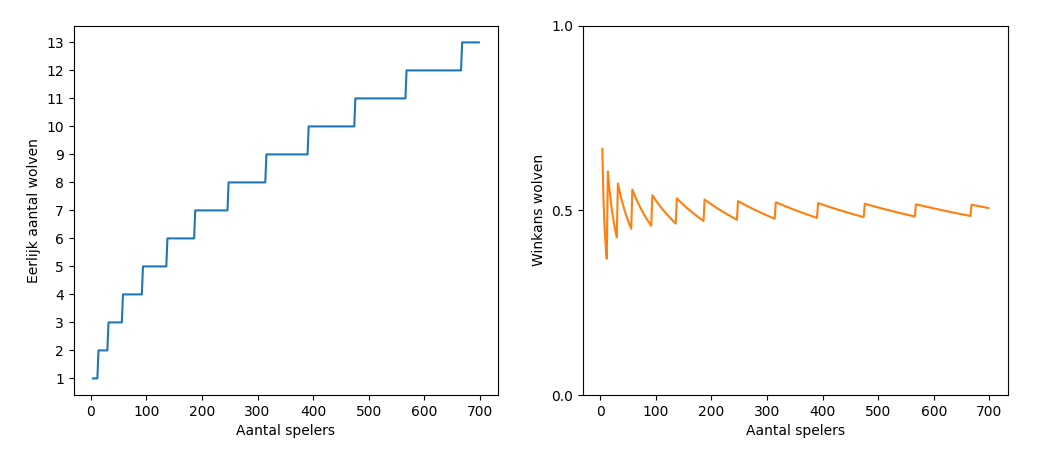
\includegraphics[width=\textwidth]{fig/res.png}
\end{center} \pause
Bij 44 spelers: 3 wolven, $P(\text{wolven winnen}) \approx 50,\!03\%$
\end{dia}

\begin{dia}{\lbt}{Complexiteit}
Het aantal \gemph{rekenstappen} $R$ (preciezer: het aantal keren dat $p(\delta, t)$ wordt uitgerekend) schaalt als
\begin{align*}
    R \approx (T_0 / 2)^2 \cdot \log_2(T_0 / 2)
\end{align*} \bigskip

\pause Dit is goed te doen voor kleine $T_0$, maar duurt te lang voor grote $T_0$ (zoals $T_0 = 8 \times 10^9$)...

\vspace{1.5cm}
\end{dia}

\begin{dia}{\lbt}{}
\vspace{2.5cm}
\begin{center}
\begin{LARGE}
\textcolor{mygreen}{Het moeilijke geval ($T_0 \gg 44$)}
\end{LARGE}
\end{center}
\vspace*{1.5cm}
\end{dia}

\begin{dia}{\lbt}{Benadering}
Bij grote aantallen spelers lukt exact oplossen niet meer, en moeten we een \gemph{benadering} gebruiken \pause \bigskip

\gemph{Aanname 1}: bij een groot aantal spelers $T_0$ kunnen we het spel benaderen met een proces dat \gemph{continu} is in $t$ \smallskip

Oftewel, een proces waarbij $P(\delta(t) = \delta)$ ook gedefinieerd is voor $t$ geen geheel getal \pause \bigskip

Waarom kan dit? \pause \bigskip

Hoe groter $T_0$, hoe langer elk spel duurt (maximaal $T_0 / 2$ stappen) \smallskip 

$\Rightarrow$ elke tijdstap is maar een relatief klein stapje
\end{dia}

\begin{dia}{\lbt}{Continue meestervergelijking}
\gemph{Idee A}: continue meestervergelijking uit statistische fysica gebruiken \pause
\begin{align*}
    P_\delta(t + \d t) &= P_{\delta + 2}(t) \, \omega_{\delta + 2 \rightarrow \delta}(t) \, \d t \\
    &+ P_\delta(t)[1 - \omega_{\delta + 2 \rightarrow \delta}(t) \, \d t]
\end{align*}

met $\omega_{\delta + 2 \rightarrow \delta}(t)$ de ``rate'' zodanig dat $\omega_{\delta + 2 \rightarrow \delta}(t) \, \d t = p(\delta + 2, t)$ \pause \bigskip

Voor kleine tijdstappen ($\d t \approx 0)$ geldt bij benadering
\begin{align*}
    \frac\d{\d t} P_\delta(t) = \omega_{\delta + 2 \rightarrow \delta}(t) \, [P_{\delta + 2}(t) - P_\delta(t)]
\end{align*}
\end{dia}

\begin{dia}{\lbt}{Continue meestervergelijking}
Voor kleine tijdstappen ($\d t \approx 0)$ geldt bij benadering
\begin{align*}
    \frac\d{\d t} P_\delta(t) = \omega_{\delta + 2 \rightarrow \delta}(t) \, [P_{\delta + 2}(t) - P_\delta(t)]
\end{align*} \smallskip

\pause Voordeel: \pause
\begin{itemize}
    \item dezelfde structuur als fundamentele vergelijking van de kwantummechanica $\Rightarrow$ oplossing bekend
\end{itemize}
\pause Nadelen: \pause
\begin{itemize}
    \item uitrekenen van oplossing in de praktijk niet sneller dan DP \pause
    \item hoe bepalen we de juiste $\omega$?
\end{itemize}
\vspace{-2mm}
\end{dia}

\begin{dia}{\lbt}{Weerwolven als Itô-proces}
\gemph{Aanname 2}: bij een groot aantal spelers $T_0$ kunnen we het spel goed benaderen met een proces dat continu is in $t$ \gemph{en in $\delta$} \pause \smallskip

Oftewel, een proces met kansdichtheid $\rho(\delta, t)$ voor $t$ en $\delta$ geen gehele getallen \pause \bigskip

Vergelijkbaar met vorige aanname: bij veel spelers verandert $\delta$ in elke stap maar relatief weinig \pause \bigskip

\gemph{Idee B}: het spel is (bij benadering) een Itô-proces
\begin{align*}
    \d \delta(t) = \mu(\delta(t), t) \, \d t + \sigma(\delta(t), t) \, \d W(t)
\end{align*}
in het domein $0 < \delta(t) < T_0 - 2t$
\vspace{-1cm}
\end{dia}

\begin{dia}{\lbt}{Weerwolven als Itô-proces}
Keuze voor $\mu(\delta(t), t)$ en $\sigma(\delta(t), t)$ volgt uit het oorspronkelijke proces: \pause
\begin{align*}
    \delta(t + 1) - \delta(t) = \begin{cases}
        -2 & \text{met kans } p(\delta, t) \\
         0 & \text{met kans } 1 - p(\delta, t)
    \end{cases}
\end{align*}
\pause \vspace{-3mm}
\begin{center}
    $\Downarrow$\vspace{-2mm}
\end{center}
\begin{align*}
    \mu &:= E[\delta(t + 1) - \delta(t))] = -2p, \\[2mm]
    \sigma^2 &:= E[(\delta(t + 1) - \delta(t))^2] - E[\delta(t + 1) - \delta(t)]^2 = 4(p - p^2)
\end{align*}
\vspace{-2mm}

\pause Bewering: kansverdelingen van beide processen naderen normaal- verdeling met gelijke gemiddelde en variantie als $T_0 \rightarrow \infty$ (bewijs?)

\vspace{-1.4cm}
\end{dia}

\begin{dia}{\lbt}{Weerwolven als Itô-proces}
In domein $0 < \delta(t) < T_0 - 2t$ geldt Fokker-Planck-vergelijking voor kansdichtheid $\rho(\delta, t)$: \pause
\begin{align*}
    \frac{\partial}{\partial t} \rho(\delta, t) = -\frac{\partial}{\partial \delta}\left[\mu(\delta, t) \rho(\delta, t)\right] + \frac12 \frac{\partial^2}{\partial \delta^2}\left[\sigma^2(\delta, t) \rho(\delta, t)\right]
\end{align*} \smallskip

\pause Analytische oplossing onwaarschijnlijk, maar numeriek oplossen mogelijk (complexiteit?) \pause \bigskip

En hoe houden we rekening met vroegtijdig stoppen ($\delta(t) \leq 0$ of $\delta(t) \geq T_0 - 2t$)? \pause \bigskip

$P(\text{wolven winnen}) = P(\text{proces stopt op } t \leq T_0 / 2 \text{ met } \delta(t) = 0)$
\vspace{-1.2cm}
\end{dia}

\begin{dia}{\lbt}{}
\vspace{2.5cm}
\begin{center}
\begin{LARGE}
\textcolor{mygreen}{Vragen?}
\end{LARGE}
\end{center}
\vspace*{1.5cm}
\end{dia}

\end{document}